\chapter{\label{cha:tool} Implementation Details}

\newcommand{\kf}{\textsc{KotFuzz}}

This chapter details the implementation of the conceptual methods
laid out in \Cref{cha:algorithm} in a system
we named \kf.
We first describe the scope of the system and its goals,
before analyzing its architecture and components.
Finally, we examine the many ways in which practitioners
can configure the system based on their individual intended use cases.

\section{\label{sec:overview}Implementation Overview}

We designed \kf~ to be a self-contained system providing tools
that (i) enable the generation of Kotlin code,
(ii) allow the differential testing of specific compiler versions,
and (iii) can perform analysis on the performance
and behavior of its algorithms.
The implementation spans around 9,000 lines of code
across five programming languages and more than dozen libraries.
In addition to providing a versatile toolkit, we aim for
\kf~ to fulfill two other key qualities.

First, \kf~ should be modular enough to allow users
to swap different components according to their needs.
Second, it should allow for a large degree of reproducibility
and experimentation, as to enable further empirical research into 
automated testing of Kotlin compiler, while at the same time
allowing users to reproduce results that might be relevant to the
future of the language.
Fortunately, containerization is a technique that excels
at both distributing software in isolation and building a controlled
environment in which strict version requirements can be met.
These properties significantly lessen the burden of modularity
and reproducibility.
As a result, the entire \kf~ system makes heavy use of containerization,
both to deliver software and to empirically assess it.

\newacronym{SOA}{SOA}{Service-Oriented Architecture}

\section{\label{sec:architecture}Architecture of the System}

The ambitious and varied tasks that \kf~ sets out to accomplish
require a versatile architecture that encourages modularity
and extendability.
For this reason, we design \kf~ to follow a \gls{SOA}.
The service-centric model allows for the separation of
individual tasks into self-contained components, called
\textit{services}, that can interface with each other
through APIs.
This is especially desirable for our system, as separating between
fuzzing, done in Java and Kotlin, embedding, performed by a Python
wrapper over \textsc{CodeBERT}, and analytics software, written
in Bash, Python, and R would present a sizable challenge
without this separation.


\begin{figure}[t]
\centering
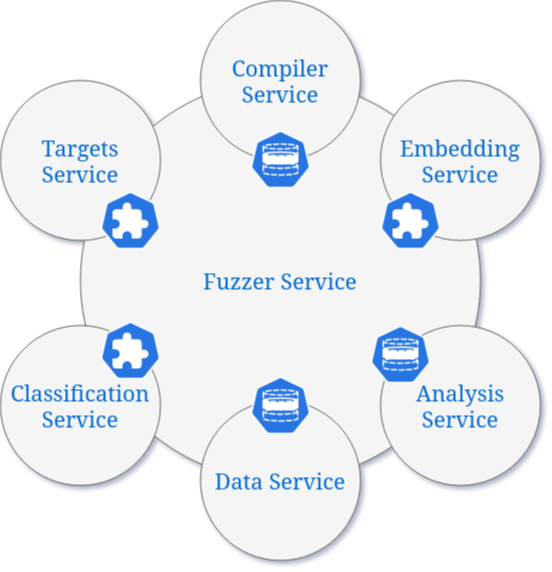
\includegraphics[scale=0.3]{img/services.png}
\caption{Service-Oriented Architecture of \kf.}
\label{fig:services}
\end{figure}

The organization of services within \kf~ is not symmetric,
instead revolving around the main fuzzer service, which implements the
theoretical methods proposed in the previous chapter.
In support of this main component are six additional services, which the remainder of
this section describes more closely.
\Cref{fig:services} depicts the overall architecture, with the six complementary
services orbiting around the fuzzer.
Services communicate either through REST APIs (denoted by puzzle pieces),
or by shared volumes, depending on the use case.
All services belong to otherwise isolated containers.

\subsubsection{Fuzzer Service}

The fuzzer service is tasked with running the generative fuzzer,
and contains the implementation of both the syntactic and semantic interfaces,
as well as the generative heuristics proposed in \Cref{cha:algorithm}.
This implementations spans circa 8,800 lines of code split between
Java and Kotlin.
Java is the main language of the fuzzer, which we chose due to previous experience, as well
as interoperability with Kotlin, which enables the usage of several libraries
developed as part of the Kotlin specification.
One such library is \texttt{grammar-tools}\footnote{https://github.com/Kotlin/grammar-tools},
a collection of tools that can parse and interface between \textsc{antlr4} and
an intermediate parse tree representation.
This is crucial for the context extraction step described in \Cref{sec:context}.

The fuzzer service is internally structured in alignment with
the sections of \Cref{cha:algorithm}.
\Cref{fig:fuzzercomp} provides a UML visualization
of the component-level composition of this service.
The center runner block is the user-facing interface
of the service, which processes command line arguments
provided by users and configures the appropriate internal state.
Three additional components implement the context, grammar,
and generative heuristic modules of the fuzzer.
A final configuration component is responsible for allowing
users to fine-tune the behavior of the fuzzer according to their goals.
The remainder of this subsection briefly details the most important
aspects of each module.

The context component is tasked with extracting relevant structural
information from a provided collection of Kotlin
files and providing a semantic interface to the fuzzer
at runtime.
The default context uses a subset of Kotlin built-in and standard library types,
including numerical and string types, exceptions and throwables, and container type interfaces.
Though limited, this subset suffices to grasp the effectiveness of the fuzzer prototype
and establish the properties of the proposed heuristics.
The fuzzer is internally able to parse a much broader and generalizable subset
of the Kotlin language, including (nested) classifier types
and their members, functions, annotations,
and visibility and inheritance modifiers.
However, due to the relatively costly nature of implementing sound
semantic constraints for all constructs of the Kotlin language,
sampling within this research prototype
is limited to a functions, expressions, and statements.

By default, we use the standard specification of \textsc{antlr4}
lexer and parser grammars. \footnote{https://kotlinlang.org/docs/reference/grammar.html}
The grammar component of the fuzzer traverses the graph representation
of the \gls{CFG} and transforms each node into its extended counterpart
as established in \Cref{sec:syntax}.
We envision that users can provide a target
node for sampling from this transformed \gls{CFG},
however, for the scope of this research prototype,
we restrict the samplable nodes to functions in the top-level
scope of a file.
We selected this option because functions are powerful constructs in Kotlin,
stressing many components of language such as name and scope resolution, type constraints,
and parameter matching.
Functions also behave as dictated by the grammar, and can contain
an arbitrary number of expressions and statements in their bodies.

\begin{figure}
%\centering
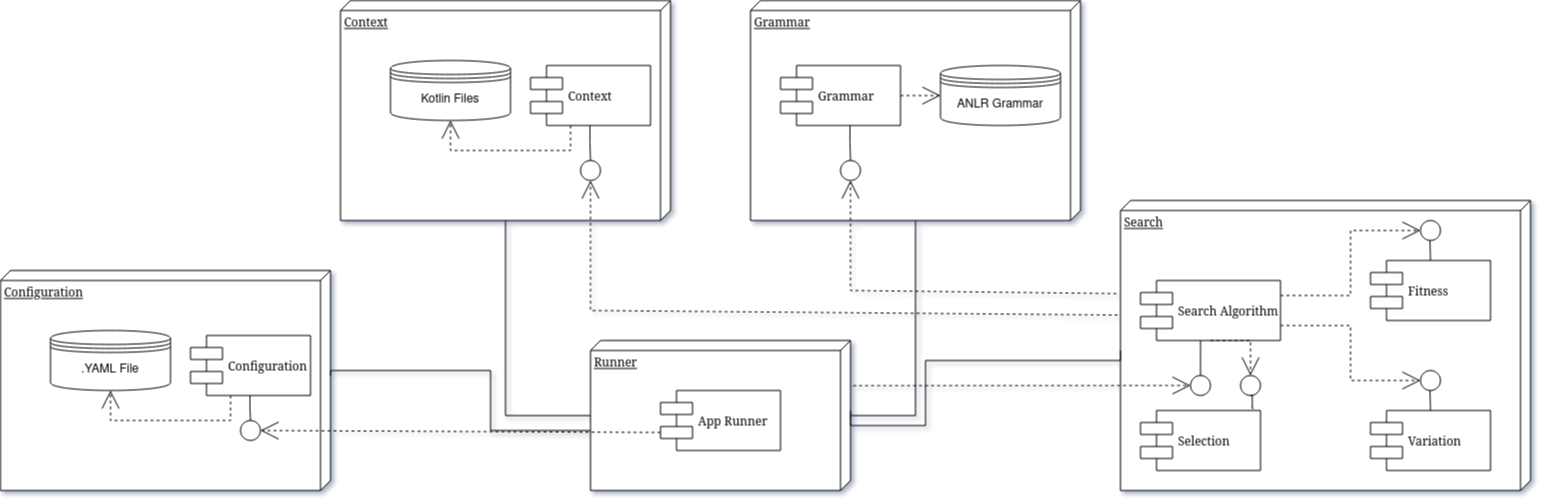
\includegraphics[scale=0.3]{img/components1.png}
\caption{Component diagram of the \kf~ fuzzer service.}
\label{fig:fuzzercomp}
\end{figure}

The search component of the fuzzer service implements both the genetic representation
of code snippets, as well as the generative heuristics built on top,
as per \Cref{sec:repr} and \Cref{sec:heuristics}.
For the latter, standard interfaces model common elements
shared throughout algorithms, including 
\gls{SO} and \gls{MO} fitness functions, selection and variation operators,
and block generation.
This enables a large degree of configurability and extendability,
as common procedures likely to be used in most algorithms
are already implemented in basic \gls{GA} classes.
Implementing novel algorithms that conform to a somewhat 
standard \gls{GA} structure is straightforward within this framework:
in most cases a developer simply needs to implement a novel \texttt{FitnessFunction}
class, choose one of the five provided selection operators, and
optionally implement a novel iteration loop.

One notable extension of this framework is the inclusion of a \texttt{RemoteEvaluation}
fitness function interface.
This interface extends its base (local) counterpart,
but allows the fuzzer to determine the fitness of individuals through HTTP requests
to remote services.
Such methods greatly increase the flexibility of the tool,
allowing remote applications to implement tailored evaluation procedures
that would otherwise prove challenging to integrate in the main service.
The embedding-based proximity optimization algorithm discussed in \Cref{subsec:proximity-ga}
is an example of such a use case.

Finally, a configuration component parses and interprets a user-provided file
that governs the behavior of nearly every aspect of the fuzzer.
We delve into the details of configuring \kf~ in \Cref{sec:configuration}.

\subsubsection{Data Service}

\newacronym{DPVC}{DPVC}{Data Packed Volume Container}

The data service is an auxiliary component of \kf~ that hosts
a large amount of data pertaining to adjacent services.
This data includes the compiler versions utilized in the compiler
and analytics services and the pre-processed Kolin files
that serve as targets for proximity optimization.
This component is part of the \gls{DPVC} design pattern
that several services adhere to,
thus increasing the amount of data cached and shared between
services, without requiring multiple processing pipelines.

\subsubsection{Embedding Service}

The embedding service is at the core of the proximity heuristics
formulated in \Cref{subsec:proximity-ga}.
This service contains a custom object that wraps the
\textsc{CodeBERT} model and allows the embedding of arbitrary pieces of text.
The text is first split and tokenized,
before the model performs a forward part 
on the tokens, retaining their embeddings.
To further allow the user to customize \kf, we
do not limit the model selection to just \textsc{CodeBERT}.
Instead, we allow the user to inject models of their choice
by mounting different volumes in the embedding container.
By default, the container running this service
shares volumes with the data service, where the default
model resides.

The main fuzzer service makes use of embeddings
by utilizing a REST API implemented through \texttt{FastAPI}
\footnote{https://fastapi.tiangolo.com/}, a popular Python library
for building lightweight and performance-oriented APIs.
The API provides two endpoints: one for embedding a single file,
and one for returning an annotated list of files.
The latter is used more frequently within proximity \gls{GA}s,
as it requires less traffic between services and reduces overhead.
To avoid costly re-evaluations of blocks,
all algorithms that rely on remote evaluations maintain
a local cache of previously considered individuals,
further reducing connectivity traffic.

\subsubsection{Targets Service}

Like its embedding counterpart, the target service supplies
critical information to the proximity-based \gls{GA}s.
This service performs two key tasks.
First, it uses the embedding service to compute numerical representations
of all test programs available in the Kotlin repository.
Second, a it uses a custom object to wrap standard clustering algorithms that
help reduce the shear number of targets.
The latter step operates in the embedding space,
and uses standard clustering algorithms implemented in the 
\texttt{skelarn} \footnote{https://scikit-learn.org/stable/modules/clustering.html}
Python library to construct a cluster structure around the projected points.

Once established, the cluster structure provides either an implicit
or explicit list of \textit{centroids}.
Some algorithms, like \textit{k-means} do so directly, while others, 
like \texttt{BIRCH} \cite{zhang1996birch} and \texttt{OPTICS} \cite{ankerst1999optics}
require and additional step to infer the underlying centroids based on the data.
In the latter case, we first run all projected points through the
inferred cluster structure and assign
each point to a cluster (unless the algorithm rejects it).
Then, we compute the centroids of each cluster as the mean
of all points assigned to it.
Whether implicit or explicit, the emerging centroids
serve as targets for the proximity optimization \gls{GA}.

Also similar to the embedding service is the targets services's
cofngiurability.
By default, we provide six clustering objects that users of
\kf~ can select from.
We selected these objects based on (i) the scalability of the
underlying \texttt{sklearn} algorithm and its ability
to handle the vast amount of test data, (ii) the centroid's retention
of the original directory structure within the Kotlin repository, 
and (iii) the number of centroids.
Most notable is the second property, which serves
as a heuristic evaluation criterion.
We score each model based on (i) the percentage of files that belong to the 
same directory in the Kotlin repository and also belong to the same cluster in the model
and (ii) the percentage of files in different directories, also assigned to different clusters.

\newacronym{DVC}{DVC}{Data Version Control}

Through this evaluation, we opt for several k-means models, which offer a good
trade-off between mirror the original directory structure and allowing
the selection of an intended number of targets (centroids).
However, we also provide several additional models as default options within this service.
Unlike the embeddings service, there is no additional implementation requirement
to extending the targets functionality.
Users can simply inject pre-trained
clustering objects in the appropriate directory,
and the runtime \texttt{FastAPI} application handles the communication with the fuzzer service.
Finally, we employ the \gls{DVC} \footnote{https://dvc.org/doc}
system to allow practitioners to orderly
modify, update, and maintain different models.

\subsubsection{Compiler and Analysis Services}

We address the compiler and analysis services together because
of their similar roles within \kf.
Both services add auxiliary functionality to the fuzzer system
and aid in its empirical assessment.
The compiler service is the lighter of the two,
and its role is to perform \gls{DT} on the
output of the fuzzer.
To speed up analysis, we allow for this service to run asynchronously
to the main service, by sharing a volume between the two containers.
In practice, this means that the compiler service passes newly
generated files through the \gls{DT} pipeline as soon as they emerge
from the fuzzer.
This feature is desirable for extending the fuzzer and continuously assessing
its bug-finding capabilities.

The analysis service provides a more complete set of analytics
tools than its light-weight counterpart, and allows
for insightful analysis of \kf 's performance.
This service also performs \gls{DT}, however, it simultaneously
monitors the compiler process through the GNU \texttt{time}
command line utility \footnote{https://www.gnu.org/software/time/},
which captures additional details regarding speed and memory usage.
In addition, each file analyzed through this service is additionally inspected
through \texttt{detekt} \footnote{https://detekt.dev/}, a static analysis
tool for Kotlin code.
Both of these features aid in detecting patterns in the generated code,
and can help link compiler defects (or performance limitations)
to properties of source code.

Finally, the analysis service also contains utilities that
extract statistics regarding the performance of the fuzzer.
These utilities include the classification of defects uncovered
in a particular fuzzer run, as well statistical tests
that determine the relative performance of more than one runs.
Because of the more performance-intensive nature of this
service, we advise against utilizing it at the same time
as the fuzzer, as it can limit compute resources.
For this use case, the compiler service is a better fit.

\subsubsection{Classification Service}

\section{\label{sec:configuration}Configuring the Tool}
